\chapter{Design, Solution and Suggestion}

\section{System Structure}
\subsection{Flow Chart}
Below is the context model of the application:

\begin{figure}[!h]
	\centering
	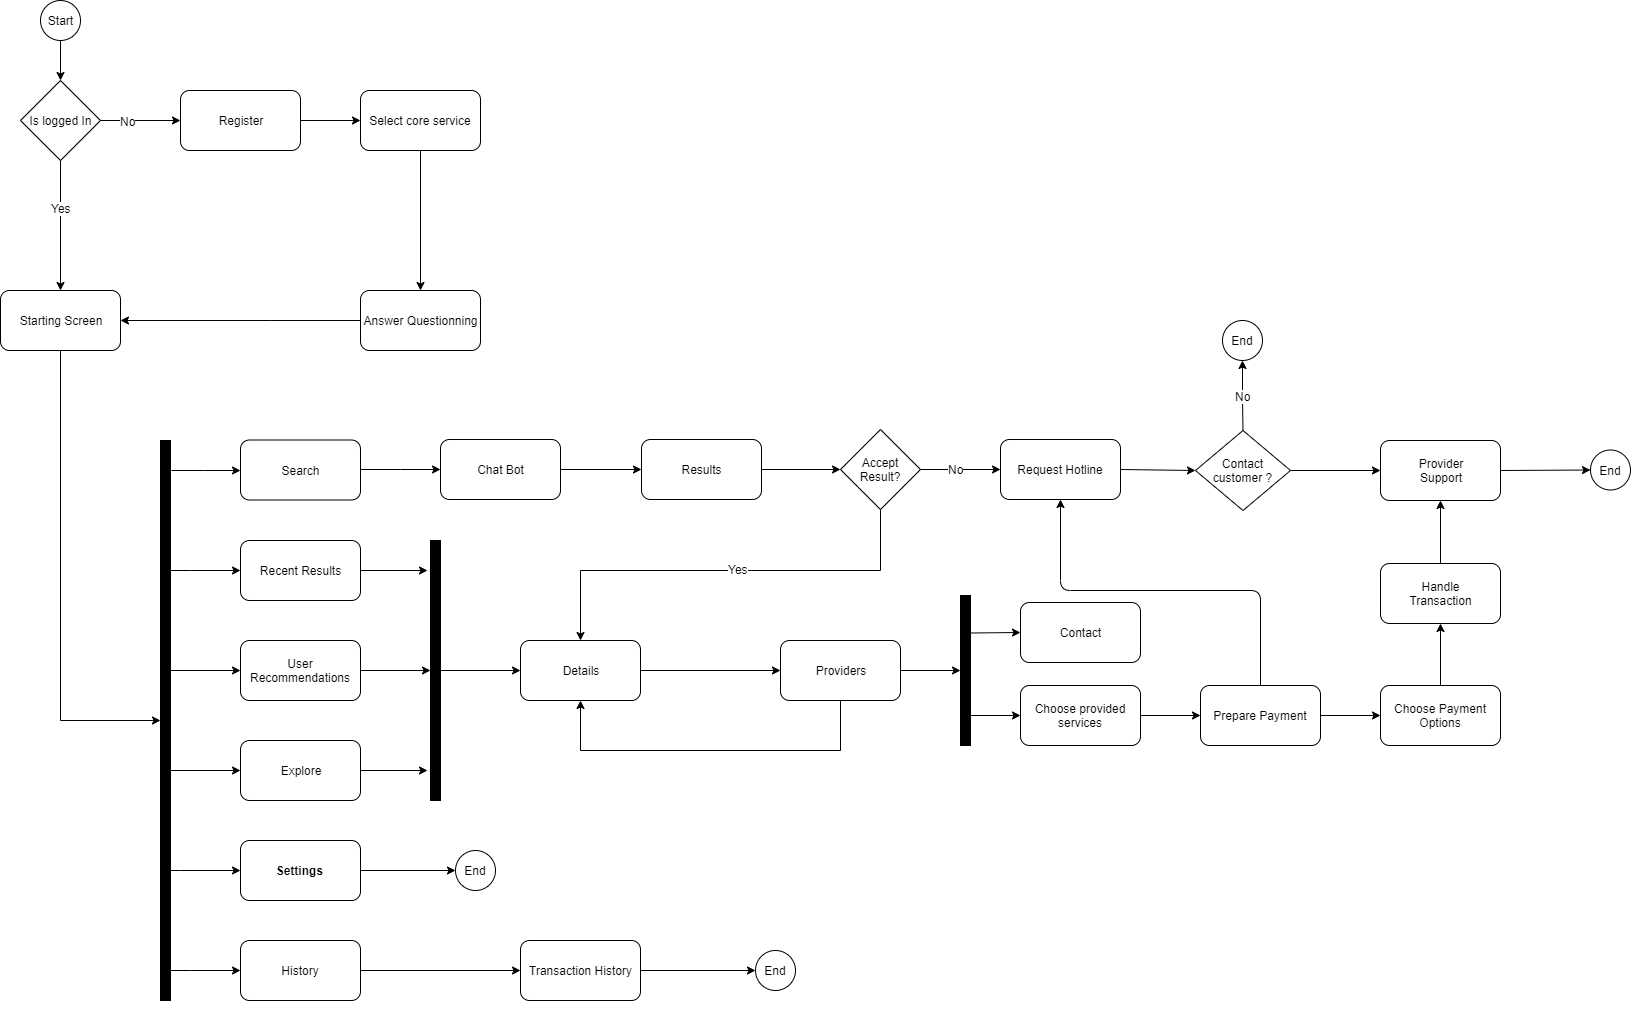
\includegraphics[scale=0.25]{Picture/architecture/context-model.png}
	\caption{Context Model of the application}
\label{fig:context-model}
\end{figure}

\section{Build a mobile application}
In previous chapter, we have discussed cross-platform mobile development which composes of
architecture of React Native, how it has the ability of running mobile in different platforms(iOS and Android)
as well as its future upgrade. 
Having thoroughly taken into consideration which mobile platforms should be applied, we finally come to React Native option
because of following reasons: 
\begin{itemize}
    \item React Native has been released for 4 years, which ensures the stabilities and huge supports from experienced communities 
    \item It inherits many great features from React core, such as components, JSX, hook,etc
    \item Its base code can be reused for web implementation. 
    \item Easy to learn and implement the project 
\end{itemize}

However, it still contains many cross-platform issues which we will discuss later. Now we discuss how we design the application's architecture that matches the business model.
Before heading to the architecture's design, we will take a look at some necessary React Native's relating components. 
Although React Native allows the communication between Javascript side and native side (iOS and Android) which lets the native side execute Javascript logic code, it still needs others components 
which are React navigation, React Redux, local storage.\\
\subsection{React Navigation}
React Navigation is born from the React Native community's need for 
an extensible yet easy-to-use navigation solution written entirely in JavaScript 
(so you can read and understand all of the source), on top of powerful native primitives. \ref{}\\ % https://reactnavigation.org/docs/en/getting-started.html 

Most of mobile apps are not built in a single screen. In fact, they are built by a dozen of screens which are navigating by 
a router. In React Native, it is the responsibilities of React Navigation.\\

Because its main tasks are to routing suitable screens base on interactions of user or users' privilege.
To design maintainable and scalable routing system, we use tab navigation, switch navigation, stack navigation in which \\
\begin{itemize}
    \item \textbf{Stack navigation}: Basically, an application does not only have one screen, it has a set of screens which put as a stack. And when switch screens in stack navigation, the app still keeps track the previous screen
    \item \textbf{Tab navigation}: Usually, at the bottom or top of the mobile's app, there is a tab navigation which turn into another screen or a set of screens(stack navigation).
    \item \textbf{Switch navigation}: Switch navigation only load one screen at time. It default resets the route when switching between screens
\end{itemize}

\subsection{React Redux}

React basically is one-way data flow. Hence, it become more cumbersome when the app is larger. As shown in picture \ref{fig:React-compare-redux}
, To access to the data of root node, it needs to pass through many layers of components which leave burdens on intermediary components. With React Redux,
it remove state management out of the Virtual DOM, we do not need to access parent's state by passing props through layers of layers, we just need to access to Redux to get 
necessary data.\\

\begin{figure}[!h]
    \centering
    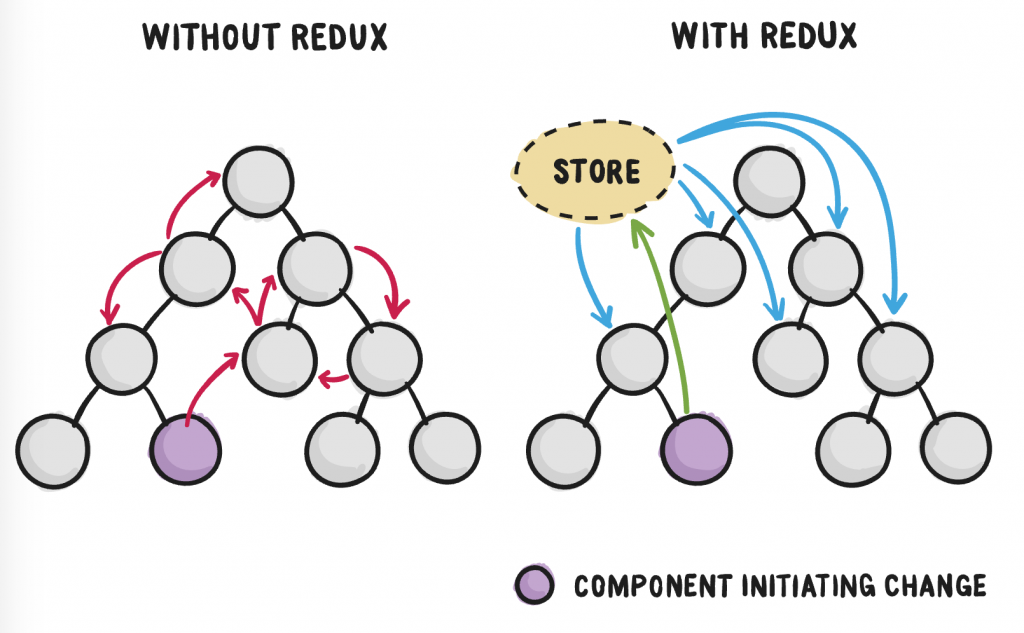
\includegraphics[scale=0.3]{Picture/mobile/RN-compare-redux.png}
    \caption{Comparison between React with Redux and React without Redux}
\label{fig:React-compare-redux}
\end{figure}

Redux is a predictable state container for JavaScript apps, which manages state in the app more effective and scalable. 
Redux can be described in three fundamental principles: \\
\begin{itemize}
    \item Single source of truth
    \item State is read-only
    \item Changes are made with pure functions
\end{itemize}

\begin{figure}[!h]
    \centering
    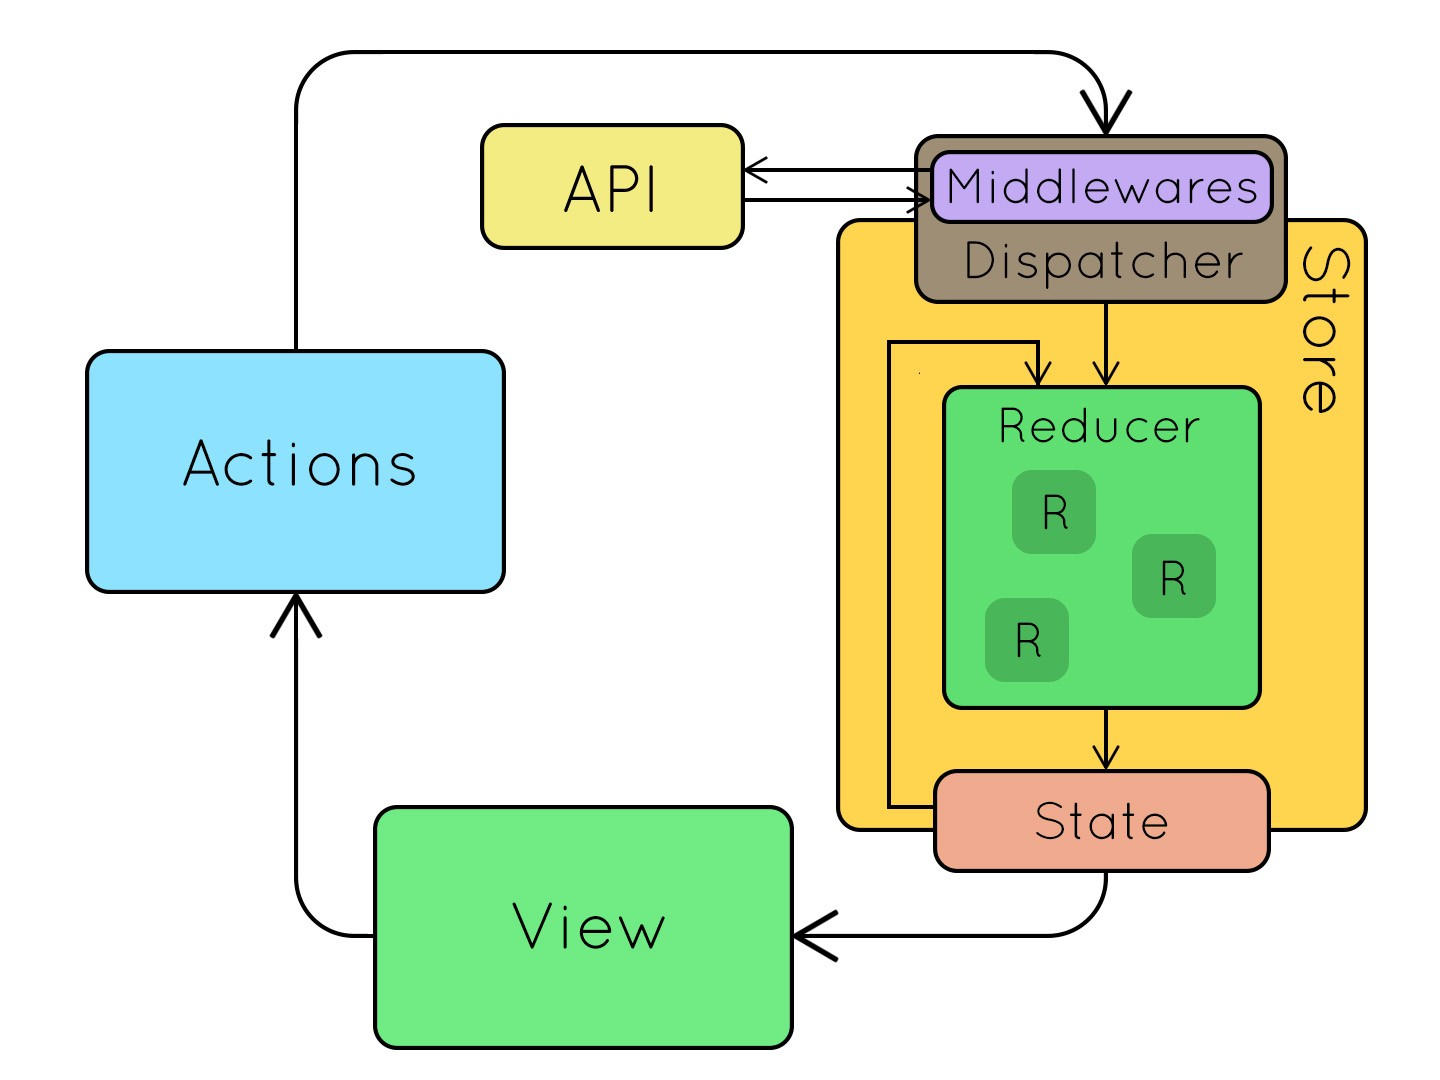
\includegraphics[scale=0.2]{Picture/mobile/React-redux.jpeg}
    \caption{React Redux flow and architecture}
\label{fig:React-redux}
\end{figure}

As specified in the picture \ref{fig:React-redux}, there are three main components in React Redux. 
\begin{itemize}
    \item \textbf{Actions}
    \item \textbf{Store}
    \item \textbf{Reducers}
\end{itemize}

% \subsection{Local storage}

% \subsection{Functionalities}
% \subsubsection{Authentication}
% \subsubsection{Chat bot}
% \subsubsection{Recommendation}

% \subsection{User interface}

\section{Build a backend server}
\subsection{System Design}
The system consists of 4 services:
\begin{itemize}
    \item Main server that accepts incoming requests, and also to host an admin application, where new information can be added.
    \item Authentication server, which handles user registration and sign in/sign out
    \item Rasa chatbot, which acts as the virtual assistant
    \item A custom action server, which handles dialogue actions that Rasa Core sends over
\end{itemize}
The services communicate using message passing via a message broker, implemented with \textbf{Redis} -- a fast in-memory key-value database, except for Rasa server, which only supports WebSockets (which is not suitable for our intended application) and HTTP.

The database used is \textbf{MongoDB}, a document-oriented database. It uses JSON-like documents with schema, and is classified as a NoSQL database. We choose it as it allows us to be more flexible with design, and support for ad-hoc queries.

Below is the architectural design of the system:
\begin{figure}[!h]
	\centering
	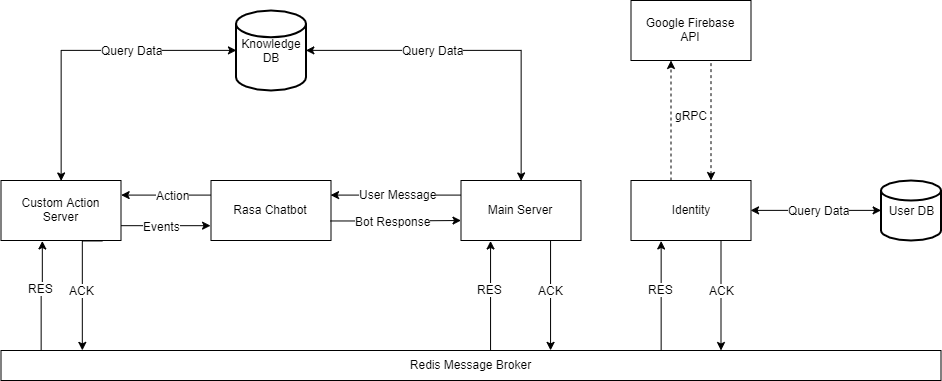
\includegraphics[scale=0.4]{Picture/architecture/System.png}
	\caption{Architecture of the application}
\label{fig:arch-design}
\end{figure}

\subsection{Communication between Services}
The subsystems communicate using message passing, using a message broker implemented in Redis, using its PubSub (Publish/Subscribe) feature.

In this system, the services subscribe to a particular \textbf{message pattern}, when another service publish a message with that pattern, the subscribed service will take that message and handle it.

\begin{figure}[!h]
	\centering
	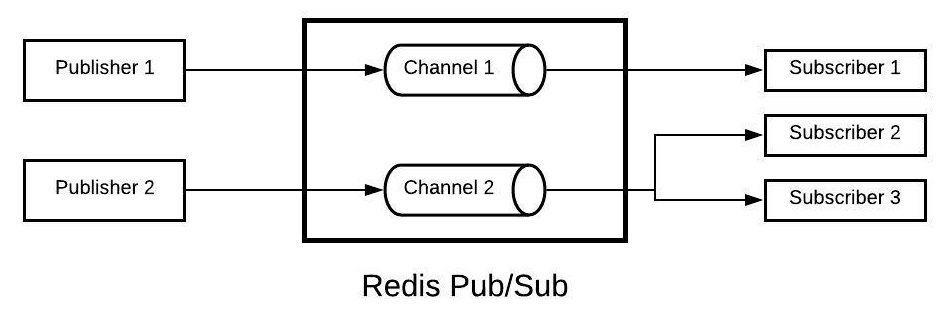
\includegraphics[scale=1]{Picture/architecture/redis-pub-sub.jpeg}
	\caption{Redis Pub/Sub Message Broker system}
\label{fig:pubsub}
\end{figure}

In our system, a service will:
\begin{itemize}
    \item Subscribe to a Redis pub/sub channel named \texttt{pattern\_ack}
    \item Publishes to channel \texttt{pattern\_res}
\end{itemize}

Below is an example of a message:
\texttt{\{"id":"68950cb0-397b-43b3-bf03-9c5f8aa619fa"\\,"pattern":"user\_create","data":"..."\}}

By using a message broker, we don't have to worry about how these subsystems communicate. However, this is indeed a central point of failure, however, there are multiple cloud providers of Redis with guaranteed reliability.

\subsection{Custom Action Server}
\subsubsection{Extending Rasa Core}
By its own, Rasa Core can only executes simple actions - replying users with text, images, etc. Some actions (e.g. database query, API calls) cannot be handled within Rasa core, and it will have to call an external server to execute these actions.

Rasa Core does this by sending a HTTP POST request to this action server, and the result of this action is an array of events, which will let Rasa Core determine the next action when it receives the response.

\subsubsection{Algorhitm}
The steps to handle these actions are as follow:
\begin{enumerate}
    \item Extract action name from request
    \item Get injected service with same action name
    \item Executes method \texttt{execute}, which will return an array of events
    \item Prepare a response containing these events and send it back to Rasa Core
\end{enumerate}

We propose a design for these custom actions, as follows:
\begin{figure}[!ht]
    \centering
    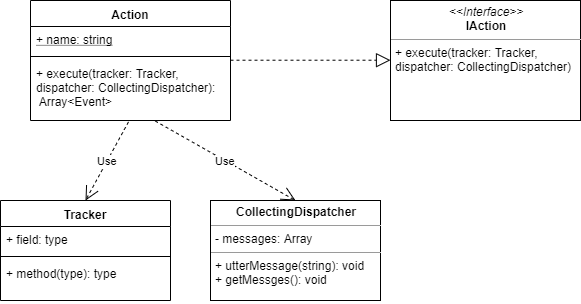
\includegraphics[scale=0.5]{Picture/architecture/Actions.png}
    \caption{Actions Class Diagram}
\end{figure}
All actions will inherit base class \texttt{Action} and implements the interface \texttt{IAction}, and will override the \texttt{execute} method, which will executes some code and emits new events to Rasa core by sending back a reply in JSON.
